% Let's start this dissertation....

\chapter{Introduction}\label{chap1}
% A '%' character causes TeX to ignore all remaining text on the line,
% and is used for comments like this one.

\fixchapterheading % Use this if section follows chapter immediately
\section{A Section}  % Produces section heading.  % level 2

Stuff.\cite{Holt:2008}

\subsection{A Subsection}   % level 3

More Stuff.\footnote{This is a footnote.} See Fig. \ref{fig:example}.


\subsubsection{This is a SubSubSection}


%% Below is a sample of image insertion. Note that there is no extesion 
%% on chap1img/example (which is really 'example.eps' and would be located 
%% in the 'chap1img' folder in this directory. Image format and file extension 
%% are assumed depending on what you compile to: 
%% ps or dvi => '.eps'; pdf => '.jpg;.png;.gif'

\begin{figure}[p]
	\begin{center}
    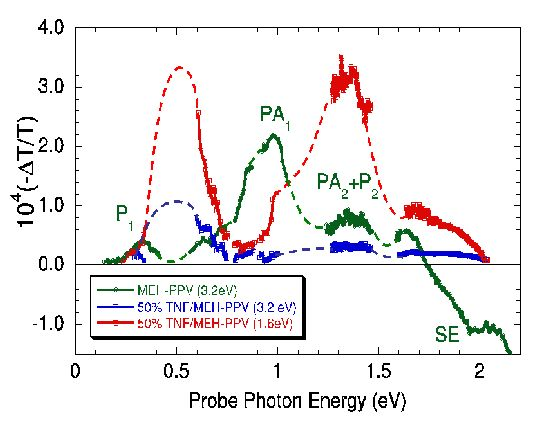
\includegraphics[width=\textwidth]{chap1img/example} 
    \caption{\label{fig:example}Caption.}
    \end{center}
\end{figure}
